\documentclass{xcpczh}
\usepackage{ctex}
\usepackage{caption}
\usepackage{subcaption}
\usepackage{geometry}
\usepackage{boxedminipage}
\usepackage{makecell}
\usepackage{xcolor}
\usepackage{tabularx}
\geometry{a4paper,scale=0.8}
\usetikzlibrary{patterns}
\schoolshort{JSUT}
\schoolname{江苏理工学院}
\location{江苏·常州}
\logo{jsuttext}

\begin{document}
	\pagestyle{empty}
	
	\begin{center}
		\vspace*{12em}
		
		\begin{figure}[htbp]
			\centering
			\begin{minipage}[t]{0.48\textwidth}
				\centering
				\icpclogo{0.15}
			\end{minipage}
			\begin{minipage}[t]{0.48\textwidth}
				\centering
				
\includegraphics[width=6cm]{jsuttext}
			\end{minipage}
		\end{figure}
		
		{\LARGE\bf 2025 \schoolshort Collegiate Programming Contest\\\schoolname\\\vspace*{1em}\location}
	\end{center}
	\tableofcontents
	\clarification{热身赛}
	\clearpage 
	\pagestyle{fancy}
	\begin{problem}{我要 AK 江苏理工学院程序设计竞赛}
		\begin{boxedminipage}[c][1.5cm][t]{22em} 
			时间限制: 1 second
			
			内存限制: 256 megabytes
		\end{boxedminipage}
		
		欢迎来到 JSUTCPC!
		
		AK 的意思是``All Killed'',表示比赛的所有题目都通过。Timothy 希望大家不仅能在未来的每一场比赛中``AK'',还能``AK''生活中的所有烦恼。感谢大家参与 JSUTCPC!
		
		所以 Timothy 认为字母表中 A 到 K 的所有字母都是幸运字母,JSUTCPC 之后的各场比赛出题人肯定不会让你``AKll,所以你需要判断他们给出的字母是否是幸运字母。
		
		\begin{inputdes}
			第一行给出一个大写字母c(c为A到Z的大写字母,不包含A和K),表示出题人给出的字母。
		\end{inputdes}
		
		\begin{outputdes}
			如果 c 是幸运字母,则输出 $\tt{true}$,否则输出 $\tt{false}$。
			
			答案不区分大小写。例如,$\tt{True}$、$\tt{TRUE}$、$\tt{TrUe}$ 和 $\tt{trUE}$ 都可能表示 c 是幸运字母。
		\end{outputdes}
		
		\section*{样例}

		\begin{table}[h]
			\begin{tabularx}{\textwidth}{|>{\raggedright\arraybackslash}X|>{\raggedright\arraybackslash}X|}
				\hline
				\textbf{输入} & \textbf{输出} \\ \hline
				\makecell[l]{$\tt{F}$} & \makecell[l]{$\tt{true}$} \\ \hline
				\makecell[l]{$\tt{W}$} & \makecell[l]{$\tt{false}$} \\ \hline
				\makecell[l]{$\tt{J}$} & \makecell[l]{$\tt{true}$} \\ \hline
			\end{tabularx}
		\end{table}
		
		\section*{注释}
		
		对于第一个样例,按字母顺序,F 位于 A 之后,K 之前,因此输出为 $\tt{true}$。
	\end{problem}

	\begin{problem}{完蛋,括号成对!}
		\begin{boxedminipage}[c][1.5cm][t]{22em} 
			时间限制: 1 second
			
			内存限制: 256 megabytes
		\end{boxedminipage}
		
		Timothy 是网络与xcpc社团的老登,他在 QQ 群里说话很奇怪,总是在一句话后面加一个括号 (。
		
		和上面一样。而且老登 Papers 说,如果 Timothy 说话时结尾的括号成对,通常是:
		\begin{enumerate}
			\item 左括号必须由相同类型的右括号封闭;
			\item 左括号必须按照正确的顺序闭合;
			\item 每个右括号都有一个与之对应且类型相同的左括号。
		\end{enumerate}
		
		如果满足以上三个条件,就说明他在开玩笑。否则,就说明他在认真说话。请帮忙判断一下 Timothy 是不是在开玩笑。
		
		\begin{inputdes}
			第一行给出一个字符串 s(s.size()$\leq 10^4$),其中仅包含字符`('、`)'、`\{`、`\}'、`[' 和 `]',确定输入字符串是否有效。
		\end{inputdes}
		
		\begin{outputdes}
			如果 Timothy 在开玩笑,则输出 $\tt{true}$,否则输出 $\tt{false}$。
			
			答案不区分大小写。例如,$\tt{True}$、$\tt{TRUE}$、$\tt{TrUe}$ 和 $\tt{trUE}$ 都表示 Timothy 在开玩笑。
		\end{outputdes}
		
		\section*{样例}

		\begin{table}[h]
			\begin{tabularx}{\textwidth}{|>{\raggedright\arraybackslash}X|>{\raggedright\arraybackslash}X|}
				\hline
				\textbf{输入} & \textbf{输出} \\ \hline
				\makecell[l]{$\tt{()}$} & \makecell[l]{$\tt{true}$} \\ \hline
				\makecell[l]{$\tt{(]}$} & \makecell[l]{$\tt{false}$} \\ \hline
				\makecell[l]{$\tt{([])}$} & \makecell[l]{$\tt{true}$} \\ \hline
			\end{tabularx}
		\end{table}
		
	\end{problem}
	
	\begin{problem}{接雨水}
		\begin{boxedminipage}[c][1.5cm][t]{22em} 
			时间限制: 5 seconds
			
			内存限制: 256 megabytes
		\end{boxedminipage}
		
		给定 $n$ 个非负整数,表示每个柱子的高度排列,其中每根柱子的宽度为 1,计算下雨后它可以捕获多少水。
		
		\begin{inputdes}
			第一行是一个整数 $n(3 \leq n\leq 3\times 10^4)$,表示柱子的数量。
			
			第二行包含 $n$ 个整数,表示柱子的高度,由空格隔开。
		\end{inputdes}
		
		\begin{outputdes}
			输出一个整数,表示能接住雨水的单位数量。
		\end{outputdes}
		
		\section*{样例}
		
		\begin{table}[h]
			\begin{tabularx}{\textwidth}{|>{\raggedright\arraybackslash}X|>{\raggedright\arraybackslash}X|}
				\hline
				\textbf{输入} & \textbf{输出} \\ \hline
				\makecell[l]{\tt{12} \\ \tt{0 1 0 2 1 0 1 3 2 1 2 1}} & \tt{6} \\ \hline
				\makecell[l]{\tt{6} \\ \tt{4 2 0 3 2 5}} & \tt{9} \\ \hline
			\end{tabularx}
		\end{table}
		
		\section*{注释}
		
		对于第一个样例,如图下所示,阴影区域是水的体积为6。
		
		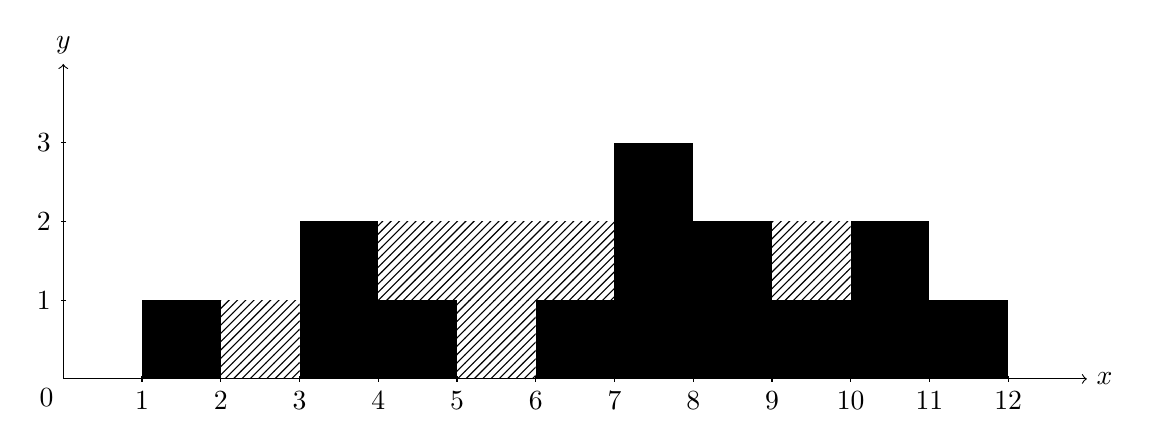
\begin{tikzpicture}
			% 绘制X轴
			\draw[->] (0,0) -- (13,0) node[right] {$x$};
			% 绘制Y轴
			\draw[->] (0,0) -- (0,4) node[above] {$y$};
			% 标注坐标原点
			\node[below left] at (0,0) {0};
			% 标注X轴刻度
			\foreach \x in {1,2,3,4,...,12}
			\draw (\x,1pt) -- (\x,-1pt) node[anchor=north] {\x};
			% 标注Y轴刻度
			\foreach \y in {1,2,3}
			\draw (1pt,\y) -- (-1pt,\y) node[anchor=east] {\y};
			
			\fill (1,0) rectangle (2,1);
			\fill (3,0) rectangle (4,2);
			\fill (4,0) rectangle (5,1);
			\fill (6,0) rectangle (7,1);
			\fill (7,0) rectangle (8,3);
			\fill (8,0) rectangle (9,2);
			\fill (9,0) rectangle (10,1);
			\fill (10,0) rectangle (11,2);
			\fill (11,0) rectangle (12,1);
			
			\fill[pattern=north east lines] (2,0) rectangle (3,1);
			\fill[pattern=north east lines] (4,1) rectangle (7,2);
			\fill[pattern=north east lines] (5,0) rectangle (6,1);
			\fill[pattern=north east lines] (9,1) rectangle (10,2);
		\end{tikzpicture}
	\end{problem}
	
	\begin{problem}{钓鱼}
		\begin{boxedminipage}[c][1.5cm][t]{22em} 
			时间限制: 1 second
			
			内存限制: 512 megabytes
		\end{boxedminipage}
		
		Timothy 和他的朋友们去岛上钓鱼。出发前,他们看了看地图。
		
		这片区域面积为$m \times n$,可以看作一个二维数组。下标$(i, j)$处的整数$t_{ij}>0$表示该区域为水域,且有$t_{ij}$条鱼;如果$t_{ij}=0$,则表示该区域为陆地。
		
		Timothy 可以从任意水域网格$t_{ij}>0$出发,进行任意次以下操作:捕获网格$(i, j)$处的所有鱼,或者移动到相邻的水域网格。
		
		Timothy 最多能捕获多少条鱼?
		
		
		\begin{inputdes}
			第一行包含两个整数 $m,n$,表示 $m\times n$ 个区域。
			
			接下来的 $m$ 行,每行 $n$ 个数字,表示该块水域的地图信息,其中第 $i$ 行和第 $j$ 列表示 $t_{ij}$。数字之间用空格分隔。
		\end{inputdes}
		
		\begin{outputdes}
			请输出Timothy最优策略下最多能捕获的鱼的数量。如果没有水格,请输出0。
		\end{outputdes}
		
		\section*{样例}
		
		\begin{table}[h]
			\begin{tabularx}{\textwidth}{|>{\raggedright\arraybackslash}X|>{\raggedright\arraybackslash}X|}
				\hline
				\textbf{输入} & \textbf{输出} \\ \hline
				\makecell[l]{$\tt{4\ 4}$\\$\tt{0\ 2\ 1\ 0}$\\$\tt{4\ 0\ 0\ 3}$\\$\tt{1\ 0\ 0\ 4}$\\$\tt{0\ 3\ 2\ 0}$} & \makecell[l]{$\tt{7}$} \\ \hline
				\makecell[l]{$\tt{1\ 3}$\\$\tt{1\ 3\ 9}$} & \makecell[l]{$\tt{13}$} \\ \hline
			\end{tabularx}
		\end{table}
		\section*{注释}
		
		对于第一个样例,Timothy可以从方格 (1,3) 开始,捕获 3 条鱼,然后移动到方格 (2,3) 并捕获 4 条鱼。
	\end{problem}
\end{document}